%----------------------------------------------------------------------------------------
%	PACKAGES AND OTHER DOCUMENT CONFIGURATIONS
%----------------------------------------------------------------------------------------
\documentclass[11pt, a4paper,oneside]{ctexbook}

%----------------------------------------------------------------------------------------
%	TITLE PAGE
%----------------------------------------------------------------------------------------

\newcommand*{\titleGP}{\begingroup % Create the command for including the title page in the document
\centering % Center all text
\vspace*{\baselineskip} % White space at the top of the page

\rule{\textwidth}{1.6pt}\vspace*{-\baselineskip}\vspace*{2pt} % Thick horizontal line
\rule{\textwidth}{0.4pt}\\[\baselineskip] % Thin horizontal line

{\LARGE \textbf{国际教育-小学系列} \\[0.3\baselineskip] \textbf{中文版}}\\[0.2\baselineskip] % Title

\rule{\textwidth}{0.4pt}\vspace*{-\baselineskip}\vspace{3.2pt} % Thin horizontal line
\rule{\textwidth}{1.6pt}\\[\baselineskip] % Thick horizontal line

\scshape % Small caps
\href{https://fieldworkeducation.com/about}{Fieldwork-Education}\\[\baselineskip] % Tagline(s) or further description
\href{https://fieldworkeducation.com/curriculums/primary-years}{IPC}\par % Location and year

\vspace*{4\baselineskip} % Whitespace between location/year and editors

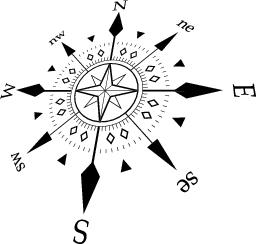
\includegraphics[width=10cm]{compass}


\vfill % Whitespace between editor names and publisher logo

{\itshape2398419426@buaa.edu.cn\par} % Editor list
{\itshape HaotianMichael \par} % Editor affiliation
\vspace*{0.5\baselineskip}
{\scshape 2018} \\ 
{\scshape Powered by \LaTeX \\[0.3\baselineskip]} % Year published

\endgroup}


\usepackage{graphicx} % Required for including pictures
\graphicspath{{Images/}} % Specifies the directory where pictures are stored
\CTEXsetup[format={\Large\bfseries}]{section}    %make section left justifing
%----------------------------------------------------------------------------------------
%       Localization
%----------------------------------------------------------------------------------------
\usepackage[UTF8,adobefonts]{ctex}
\usepackage{array, booktabs}
\usepackage{graphicx}
\usepackage[x11names]{xcolor}
\usepackage{colortbl}
\usepackage{fontspec}
\newcommand{\foo}{\color{baseD}\makebox[0pt]{\textbullet}\hskip-0.5pt\vrule width 1pt\hspace{\labelsep}}

%\setmainfont[Boldont=WenQuanYi Micro Hei]{AR PL SungtiL GB}
%\setsansfont[BoldFont=WenQuanYi Micro Hei]{AR PL KaitiM GB}
%\setmonofont{DejaVu Sans Mono}

%\XeTeXlinebreaklocale "zh"
%\XeTeXlinebreakskip = 0pt plus 1pt minus 0.1pt

\usepackage[top=1in,bottom=1in,left=1.25in,right=1.25in]{geometry}
%\linespread{1.2}

\usepackage[Glenn]{fncychap}

\usepackage{fancyhdr}
\setlength{\headheight}{15.2pt}

%----------------------------------------------------------------------------------------
%       Useful Packages
%----------------------------------------------------------------------------------------
\usepackage{color}
\usepackage{url}
\usepackage[colorlinks, linkcolor=black,anchorcolor=black, citecolor=black]{hyperref}

\usepackage{xcolor} % Required for specifying colors by name
\definecolor{ocre}{RGB}{243,102,25} % Define the orange color used for highlighting throughout the book

% BASE16
\definecolor{base0}{HTML}{181818}
\definecolor{base1}{HTML}{282828}
\definecolor{base2}{HTML}{383838}
\definecolor{base3}{HTML}{585858}
\definecolor{base4}{HTML}{B8B8B8}
\definecolor{base5}{HTML}{D8D8D8}
\definecolor{base6}{HTML}{E8E8E8}
\definecolor{base7}{HTML}{F8F8F8}
\definecolor{base8}{HTML}{AB4642}
\definecolor{base9}{HTML}{DC9656}
\definecolor{baseA}{HTML}{F7CA88}
\definecolor{baseB}{HTML}{A1B56C}
\definecolor{baseC}{HTML}{86C1B9}
\definecolor{baseD}{HTML}{7CAFC2}
\definecolor{baseE}{HTML}{BA8BAF}
\definecolor{baseF}{HTML}{A16946}
\definecolor{Gray}{HTML}{CCCCCC}
\definecolor{linkcolor}{HTML}{EC008C}
\definecolor{codecolorpink}{HTML}{CC00FF}
\definecolor{NoteColorFont}{HTML}{6D727D}
\definecolor{NoteColorLine}{HTML}{C3CAD9}
\definecolor{ExeColorFont}{HTML}{FF9900}
\definecolor{ExeColorLine}{HTML}{FFF678}
\definecolor{ExeColorBack}{HTML}{FFFFCC}
\definecolor{ThinkColorFont}{HTML}{629D81}
\definecolor{ThinkColorLine}{HTML}{93E87D}
\definecolor{ThinkColorBack}{HTML}{C1FA9B}

\usepackage{amsmath,amsfonts,amssymb,amsthm} % For math equations, theorems, symbols, etc
\usepackage{booktabs} % For tables
\usepackage{tabularx}
\usepackage{multirow} % for multiple row tables.
\usepackage{lettrine}    %expand font size 
\usepackage{indentfirst}  %indent at beginning


%\makeatletter
%\renewcommand{\section}{\@startsection{section}{1}{0mm}
%  {-\baselineskip}{0.5\baselineskip}{\bf\leftline}}
%\makeatother


%----------------------------------------------------------------------------------------
%       Some Extra Definitions
%----------------------------------------------------------------------------------------

\RequirePackage[framemethod=default]{mdframed} % Required for creating the theorem, definition, exercise and corollary boxes

% Exercise box
\newmdenv[skipabove=10pt,
skipbelow=10pt,
rightline=false,
leftline=true,
topline=false,
bottomline=false,
backgroundcolor=ExeColorBack,
linecolor=ExeColorLine,
innerleftmargin=5pt,
innerrightmargin=5pt,
innertopmargin=5pt,
innerbottommargin=5pt,
leftmargin=0cm,
rightmargin=0cm,
linewidth=12pt]{eBox}

% Thinking box
\newmdenv[skipabove=10pt,
skipbelow=10pt,
rightline=false,
leftline=true,
topline=false,
bottomline=false,
backgroundcolor=ThinkColorBack!30,
linecolor=ThinkColorLine,
innerleftmargin=5pt,
innerrightmargin=5pt,
innertopmargin=5pt,
innerbottommargin=5pt,
leftmargin=0cm,
rightmargin=0cm,
linewidth=12pt]{tBox}

% Note box
\newmdenv[skipabove=10pt,
skipbelow=10pt,
rightline=false,
leftline=true,
topline=false,
bottomline=false,
backgroundcolor=NoteColorLine!15,
linecolor=NoteColorLine,
innerleftmargin=5pt,
innerrightmargin=5pt,
innertopmargin=5pt,
innerbottommargin=5pt,
leftmargin=0cm,
rightmargin=0cm,
linewidth=12pt]{nBox}

% Boxed/framed environments
\newtheoremstyle{ocrenumbox}% % Theorem style name
{0pt}% Space above
{0pt}% Space below
{\normalfont}% % Body font
{}% Indent amount
{\small\bf\sffamily\color{ExeColorFont}}% % Theorem head font
{\;}% Punctuation after theorem head
{0.25em}% Space after theorem head	
{\small\sffamily\color{ExeColorFont}\thmname{#1}\nobreakspace\thmnumber{#2}% Theorem text (e.g. Exercise 2.1)
\thmnote{\nobreakspace\the\thm@notefont\sffamily\bfseries\color{black}---\nobreakspace#3.}} % Optional theorem note
\renewcommand{\qedsymbol}{$\blacksquare$}% Optional qed square

\newtheoremstyle{purplenumbox}% % Theorem style name
{0pt}% Space above
{0pt}% Space below
{\normalfont}% % Body font
{}% Indent amount
{\small\bf\sffamily\color{ThinkColorFont}}% % Theorem head font
{\;}% Punctuation after theorem head
{0.25em}% Space after theorem head	
{\small\sffamily\color{ThinkColorFont}\thmname{#1}\nobreakspace\thmnumber{#2}
% Theorem text (e.g. Thinking 2.1)
\thmnote{\nobreakspace\the\thm@notefont\sffamily\bfseries\color{black}---\nobreakspace#3.}} % Optional theorem note
\renewcommand{\qedsymbol}{$\blacksquare$}% Optional qed square

\newtheoremstyle{blackbox} % Theorem style name
{0pt}% Space above
{0pt}% Space below
{\normalfont}% Body font
{}% Indent amount
{\small\bf\sffamily}% Theorem head font
{\;}% Punctuation after theorem head
{0.25em}% Space after theorem head
{\small\sffamily\color{NoteColorFont}\thmname{#1}\nobreakspace\thmnumber{#2}
% Theorem text (e.g. Theorem 2.1)
\thmnote{\nobreakspace\the\thm@notefont\sffamily\bfseries---\nobreakspace#3.}}% Optional theorem note

% Defines the theorem text style for each type of theorem to one of the three styles above
\theoremstyle{ocrenumbox}
\newtheorem{exerciseT}{Exercise}[chapter]
\theoremstyle{purplenumbox}
\newtheorem{thinkingT}{Thinking}[chapter]
\theoremstyle{blackbox}
\newtheorem{noteT}{Note}[section]

\newenvironment{exercise}{\begin{eBox}\begin{exerciseT}}{\hfill{\color{ExeColorFont}\tiny\ensuremath{\blacksquare}}\end{exerciseT}\end{eBox}}
\newenvironment{thinking}{\begin{tBox}\begin{thinkingT}}{\hfill{\color{ThinkColorFont}\tiny\ensuremath{\blacksquare}}\end{thinkingT}\end{tBox}}
\newenvironment{note}{\begin{nBox}\begin{noteT}}{\end{noteT}\end{nBox}}

%----------------------------------------------------------------------------------------
%       Code Environment
%----------------------------------------------------------------------------------------
\usepackage{minted}
\usemintedstyle{manni}

% code box
\newmdenv[backgroundcolor=base7,
linecolor=baseD,
bottomline=false,
leftline=true,
rightline=false,
topline=false,
linewidth=2pt,
leftmargin=13pt]{pcodeBox}

\renewcommand{\theFancyVerbLine}{
  \sffamily
  \textcolor{baseB}{\arabic{FancyVerbLine}
  }
}

\usepackage{caption}

%\captionsetup{type=codeCaption}
\newenvironment{codeBox}{\begin{pcodeBox}\fontsize{9pt}{9pt}}{\end{pcodeBox}}
\newenvironment{codeBoxWithCaption}[1]{\begin{pcodeBox}[frametitle={\captionof{listing}{#1}\color{base6}\rule{\textwidth}{0.7pt}}]\fontsize{9pt}{9pt}}{\end{pcodeBox}}

\BeforeBeginEnvironment{minted}{\begin{codeBox}}
\AfterEndEnvironment{minted}{\end{codeBox}}

%----------------------------------------------------------------------------------------
%       Lists
%----------------------------------------------------------------------------------------
\usepackage{enumitem}
\setlist[description]{labelindent=22pt} 

%----------------------------------------------------------------------------------------
%       Main Body
%----------------------------------------------------------------------------------------
\begin{document}

\pagestyle{empty} % Removes page numbers
\titleGP % This command includes the title page

\frontmatter
\pagestyle{plain}
%\chapter{译者序}


\subsection{关于FIELDWORK-EDUCATION}
     \lettrine[lines=1]{F}{IELDWORK-EDUCATION}本身是一家为学校提供专业、适用和实时的国际化教育机构\footnote{在标题页有该网站链接},创立于1984年。该机构目前有为学校提供学前、小学、中学的国际课程。\par

\subsection{关于IPC}
     \lettrine[lines=2]{I}{PC}全称International Primary Curriculum。国际小学课程,是FIELDWORK-EDUCATION为小学生提供的课程。主要受众是5-11岁的小学生。\par

\subsection{关于本次翻译}
     \lettrine[lines=2]{本}{次翻译工作}我们将每一单元的翻译作为一个Project,每一个项目分为排版和翻译工作两部分,排版使用\LaTeXe,翻译为人工翻译。全书按照原版的目录索引以章节作为单位进行翻译。每一个项目的源代码和源文件都作为模板托管在\href{https://gitlab.com/haotianmichael/LatexTemplate}{GitLab}上。\par
     
     


    

\frontmatter
\tableofcontents


\mainmatter
\pagestyle{fancy}
\chapter{基本信息}
    这一部分详细介绍了本单元学习的时间分配,和其他课程的联系以及教学目标的评价。

\section{时间分配}
    本单元的学习预计会持续大约3周的时间。
    下面的时间分配表仅仅作为参考,具体细节和每一个学校自己的教学计划和内容有关。


\begin{table}[h]     
\begin{tabular}{l|l|l}
\hline
\colorbox[gray]{0.95}{ & 小时数 & 周数 } \\
\hline
学习入口、获取知识、主题阐述 &  4 & 1\textbackslash2 \\
灵感单元的学习  & 16  &   2  \\
学习出口  & 4  &  1\textbackslash2 \\
\hline
\end{tabular}
\end{table}



\section{和其他IPC课程的联系}
    本单元课程的学习并没有突出什么主题,因此是独立于其他IPC课程目标存在的。下面是本单元独立于其他主题的教学目标。
    孩子们将会:
    \begin{itemize}
      \item 了解到最新的关于大脑和学习的一些研究和资料 
      \item 掌握自己的行为是如何影响自身的学习效果的
      \item 能够将所学到的理论知识运用到自己的学习中并思考这样做的结果
    \end{itemize}


\chapter{学习目标}


\section{脑波单元的学习目标}
\footnote{这里和1.2部分重复}孩子们将会:
      \begin{itemize}
        \item 了解到最新的关于大脑和学习的一些研究和资料 
        \item 知道大脑的组成部分及其功能
        \item 了解学习的不同方式  
        \item 了解一些如何提高学习技巧和学习态度的知识
        \item 了解在学习过程中合作和全球化意识的重要性
      \end{itemize}  
 

\chapter{学习评估}
    您的孩子每天是不是把几乎所有的时间都花在学习上?\par
    当学习完这个主题单元\footnote{指灵感-单元}的内容之后,我们希望在以后每一个单元的学习过程中都能够回答这样一个问题————我们的孩子在学习能力上有哪些提高? \par
    我们总结了关于学习能力三个需要思考的领域和三种需要评价的学习类型。 \par

\section{三个领域:学术、私人和国际}
    这三个领域分别为:学术圈、私人领域和国际化的场景。要完成对这三个领域的思考,你需要访问IPC关于每一个主题的学习目标(包括国际化的内容)和IPC课程的个人目标————该列表可以在\href{https://members.greatlearning.com/ipc/documents?category=31}{IPC实施文件}的附录A中找到。当然你也可以在会员区的\href{https://members.greatlearning.com/ipc/assess/learninggoals}{评估部分}找到IPC学习目标比较完整的版本。


\section{三种类型:知识、技能和理解}
    这三种类型包括知识、技能和理解。我们相信区分这三者对孩子学习的发展至关重要。我们还认为知识、技能和理解力三者都有其独特的特征,这些特征会影响每一个人的计划、学习、教学、评估和报告方式。从这个角度看,这些特征之间的不同含义影响是深远的,并值得进一步的思考。


\subsection{知识}
    \textbf{知识}指的是真实的信息。尽管要回忆起这些知识并不是简单事,但相对来说知识本身是比较容易能够传授和评估的(通过智力测试、课堂测试、单项选择等)。你可以要求孩子们去研读需要学习的知识,但是你也应该告诉他们那些他们需要知道的知识。知识本身是不断更新迭代的,这对于学校来说是一个挑战,因为学校必须能够选择在特定的一段时间内适合孩子们了解和学习的知识。 \par
    IPC\footnote{国际小学课程}并不提供知识评估(测试或者考试)的例子,因为IPC课程中的知识内容可以适应任何国家课程的要求。


\subsection{技能}
    \textbf{技能}指的是那些孩子们能够做的事情。技能需要在实践中学习并需要时间去掌握。技能的特点是你训练的时间越长,那这项技能你掌握的越熟练。技能也是可以传授的,往往比知识更稳定————这几乎适用于所有学校的教学科目。\par
    IPC通过\href{https://members.greatlearning.com/ipc/assess/}{IPC学习计划评估}支持学习追踪和学习评估,该计划评估的内容包括老师的评估准则、学生的评估准则和学习建议。

\subsection{理解}
    \textbf{理解}指的是对一些概念思想的逐渐把握和发展,换句话讲就是我们经常说的“灵光一现”的时刻。人的理解是不断发展的。  \par
    IPC并不能为您的孩子们评估理解力。但是课程允许您提供一整套不同的体验机制来加深孩子们的理解力。\par
    \begin{note}
      请注意: \par
      和IPC学习计划评估一样,我们还和Classroom Monitor\footnote{一家在线学习评估机构}合作推出了一套线上评估跟踪工具。关于如何注册并使用这套工具,请给\underline{member@fieldworkeducation.com}写信询问详细的信息。
    \end{note}


\section{规划评估}
     一旦你开始为各个IPC课程主题规划不同的学习目标,那在每一个单元的学习过程对评估目标进行规划也就变的很重要了。评估需要面面俱到但是也需要每一个都严格以确保孩子们学到了我们学习规划中的所有内容。下面的图表提供的一套机制或许可以帮助实现这一点。


\section{帮助孩子们自己评估自己的学习}
     除了教师的评估之外,让孩子们自己参与整个评估过程并据此设定下一步的提高方案也是至关重要的。让孩子们对每一个单元的学习做出自我评估(使用学生评估准则来评价技能,使用学校提供的其他方式来评估知识和理解力)。  \par
     他们可以使用下面的标题来列出新学习的知识,技能和理解。
     \begin{itemize}
       \item 我现在知道的新事物
       \item 我现在可以做的新事情
       \item 我现在开始理解的新概念
     \end{itemize}   \par
     从学习过程中的不同角度和方面记录孩子们对自己的评估:
     \begin{itemize}
       \item 哪一方面做得比较好?
       \item 哪些方面是下次有机会提高的,方法是什么?
       \item 哪些方面是最最有趣的? 
       \item 更喜欢如何学习——独自,两个人,小组,人多一些的组还是整个班级?
       \item 更喜欢哪一种学习和记录的方式——记笔记、讨论还是动手实践?这项评估也可以支持IPC课程中的个人目标发展。
     \end{itemize}  \par
    

\section{更多信息}
     想要了解到更多的关于知识、技能和理解评估的信息,请访问:
     \begin{itemize}
       \item  \href{https://members.greatlearning.com/ipc/documents?category=31}{IPC实施档案}
       \item  \href{https://members.greatlearning.com/ipc/assess/aflfile}{学习评估实施档案}
       \item  \href{https://members.greatlearning.com/ipc/bottomline9/}{IPC自我反省程式}
     \end{itemize}  
     \par
     或者直接联系团队:\underline{member@fieldworkeducation.com}

\chapter{学习入口}
    让同学们想一些自己比较擅长的事情。完全可以是课堂之外的事情。如果有同学提到了比如艺术、体育、音乐、电脑游戏这些外延比较宽泛的领域,让他们描述的更清楚一些。因为可能需要他们将自己的技能和知识教给别人。\par
    给每一个同学一张卡片,每一位同学可以在上面写上他们的名字和他们能够教给别人的东西比如:"40米开外的铅球扔法"、“站在别人的头上”、“同时玩4个球”、“如何同时快速得出两个数的乘积“……或许同学们的想法会更加奇特和有意思,老师在筛选的时候需要保证最基本的安全。\par
    告诉同学们他们即将成为别人的老师,将自己的高超技术传授给别人。将同学两人分组,这样每一位同学既是老师又是同学。例如,老师可以从帽子中抽出卡片,将它们显示在墙上并邀请同学们随机选择。\par
    首先留时间给同学去思考他们已经学习过的关于快速学习和快速教学的知识,然后收集每个人的观点,以这些为基础来规划教学。可以从这几个方面作出提示:\par
    \begin{item}
      \item 和教学内容相关的知识、技巧和理解。应该如何具体辨别和掌握?
      \item 老师的各种教学方法————老师会给学生提供什么阅读材料(比如帮助手册)、提供什么示范(建模)、会有什么具体的课堂展示(比如PPT)或者以上三者都有?
      \item 对学习者有利的事情————他们使用的语言、如何调整出他们的积极心态?这些和我们已经学过的关于学习的知识有什么联系?
      \item  学习评估————学习者如何知道他们是否进步?我们如何监督他们的进度并根据实际情况提供帮助?学成的标准具体会是什么?\footnote{这也是任务的一部分,学生们必须得自行设计自己的评估准则。不过学生可以参考他们已经很熟悉的IPC学习计划评估。如果学校并没有使用这套计划,那学生可以考虑自行简化和修改学校的学习评估系统。IPC评估准则一共有三个阶段:初学、一般和精通。希望这些可以帮助学生自行设计出自己的评估准则。(IPC准则可以再哎会员区下载)} 
    \end{item}
    \par
    固定时间让学生们设计和准备他们即将需要教授的内容。并且需要考虑到他们上课时候需要用到的道具。\par
    老师需要将学习入口上课时间划分为两部分。这样第一部分结束之后学生还可以有足够的时间去准备和配备他们上课需要的装备、材料和教学资源。他们的学习过程和教学过程也会非常顺利。\par
    一旦学生准备好,两人分组开始第一部分:\par
    给同学们最多1小时时间来实施完成第一部分的教学和学习。然后两人身份交换,老师成为学生;学生成为老师。给另外一小时进行第二部分的学习和教学。在每一部分的过程中鼓励孩子们互相监督和评价学习进度——在每部分结束的时候,给双方一次机会一起完美结束。\par
    同学可能会使用自己的视角来进行监督。如果你正在使用IPC学习计划评估,那么三个阶段(初学、一般、精通)可以比做成一座高山,到达山顶就是精通。又可以看成是还在生长的大树。老师们甚至可以做一个全班同学共同的监督工具。每一位同学可以将自己的图片放到相应的阶段上。每一个人都应该确保学习并不是竞争,每一次评估将会是一次帮助我们了解我们的学习过程,我们还可以上升的领域、我们需要提高的部分的一次机会。\par
    全班一起讨论过程中到底发生了什么?你或许想画一张思维导图来记录这一切比如:\par
    \begin{item}
      \item 学习起来很容易因为……
      \item 学习起来很吃力因为……
      \item 教起来很容易因为……
      \item 教起来很吃力因为……
    \end{item} 
    问同学,如果他们即将有另一次机会来做一遍。他们希望哪里被改善来提高教学效果。\par
    学习入口的结束应该是做出一个”如何成为一个更好的老师的标准“或者”如何成为一个更好的学生准则”。然后将这两份报告贴在展示区,在接下来的一年内都可作为参考。\par
    学生们应该对学习入口的内容非常了解。但是如果你的学生是新来的,对IPC不是很了解,老师需要复习一下相关内容。每一个IPC学习主题都会有一个学习入口,学习入口的目的主要是让学习者对即将学习的主题提起兴趣,并且有一些这方面的思考。老师可以问一下学生们学习入口到底对自身的学习过程有什么正面作用,甚至有什么进一步的帮助。\par
    
    

\chapter{知识获取}
    

\chapter{全局观}
    如果巧克力种在树上那岂不是很有意思?嗯,当然很有意思。但是如果我说,我们打算去自己制作一些巧克力的话,是不是也很有意思?对!我们打算自己制作一些巧克力。而且我们还要探索关于巧克力更有趣的事情……


\include{chapter/7-ExplainingTheThem}
\chapter{知识图谱}
   


\section{可可}
     可可发源于玛雅文明,主要生长在危地马拉。是一种价值很高的商品。在加工之后,可可树上的豆子会被制作为巧克力饮品中的巧克力。想我们一样,玛雅人也喜欢巧克力,不过不同的是我们将巧克力做成巧克力棒来吃,而玛雅人是喝!他们用辣椒等香料调味巧克力饮料,有时他们会用蜂蜜。他们确保自己的音频会有很多的泡沫,我们在很多地方看到这种描述。我们也看到过一些关于玛雅人如何制作者写又泡沫的饮品————将液体从高处倒进另一个容器中。可可豆在烘烤之后,便于存储和运输。也正在因为这个原因,可可在后经济学和接触时期的巨大市场经济中成为一种很重要的交换媒介(货币)。从这个角度来讲,玛雅人实际上是在喝钱!\par
     将可可作为一种货币和饮品的传统被由中美洲和南美洲的阿兹特克人延续下来。这帮人将这种饮品成为“chocolatl”\footnote{巧克力的英文是chocolate}。该饮品被作为“神的食物”并放在金被子中作为皇家贡品。据说皇帝蒙特祖玛一天要喝50杯!可可不仅是一种很招人喜爱的饮品。更是玛雅人和阿兹特克人宗教活动和社会活动中很重要的组成部分。\par

\section{哥伦布和科尔特斯}
     16世纪的探险家哥伦布,在1504年的时候,从当时的新世界————就是现在的美洲带了一些可可回到西班牙。西班牙国王和皇后并没有认识到哥伦布带回来的这些豆子的重要性,他们倒是很看重哥伦布带回来的黄金和奇珍异宝。豆子的重要性被1519年的探险家科尔斯特发现了。刚开始蒙特祖玛国王赠予很多的可可豆,但科尔斯特并不喜欢。直到他发现这些豆子可以被作为当地的货币使用的时候(4个豆子换一只兔子,10个豆子换一个奴隶),这时候他才意识到这一发现的重要性————他可以在树上种出钱来。

\section{关于埃尔南 科尔斯特的更多信息}
     科尔斯特是一位西班牙的探险家,他在1521年的时候征服了阿兹克特王朝。科尔斯特利用自己洁白的皮肤和小胡子让蒙特祖玛二世国王相信自己就是神。上古的预言成真了。而且国王也相信了这件事情。但是之后科尔斯特并没有表现的像一个神一样。他们被驱逐出境。但是科尔斯特不久之后又回来了,这次他带了600名士兵。他捉住了蒙特祖玛二世国王并毁掉了阿兹特克王朝的首都特诺奇蒂特兰城。并在废墟上建立了墨西哥城。原始城市的所有遗迹都是主殿的废墟。


\section{巧克力酱}
     从韦拉克鲁斯到塞维利亚的巧克力官方装箱发生在1585年。在17世纪的欧洲贵族中,辣椒被替换成为糖从而变得更加流行了。英国人,法国人和德国人将这些可可引进到自己的殖民地。在美国,巧克力是在马萨诸塞州多切斯特首次制作的。第一个巧克力棒是由弗莱在1847年在伦敦制作的。两年后,吉百利制作了类似的产品。 牛奶巧克力是由Daniel Peter于1876年在瑞士制造的,只需加入奶粉即可。第一次世界大战后几年,雀巢推出了白巧克力。它含有可可脂,但根本没有可可固体。 出于这个原因,有些人认为它不应该被称为“巧克力”。今天,世界上80%的巧克力仅由六家跨国公司生产,包括雀巢,火星和吉百利。最大的巧克力消费者是瑞士,每人每年消费超过10公斤(22磅)。 排名前十位的消费者包括:瑞士,德国,奥地利,爱尔兰,英国,挪威,爱沙尼亚,斯洛伐克,瑞典和哈萨克斯坦。


\section{主打产品}
      




\section{热带生物群系}



\section{可可树}


\section{收获}



\section{}

\chapter{地理单元的学习目标}
    同学将会:\par

    \begin{itemize}
      \item 了解特定的地区是如何被人类行为干涉的
      \item 了解特定自然地区对人类的生活是如何影响的
      \item 了解自己的住宿国家的天气条件和气候条件,思考这些条件是如何影响环境和当地人的生活的
      \item 能够明白地理的专业术语
      \item 能够使用不同层面的地图进行一些特定地理特征和位置的定位和识别
      \item 能够通过第二信息源来获得地理信息
      \item 能够就一些自然环境的特征给出自己的建议和看法,并能够谈谈这些地区的环境的优化措施
      \item 能够谈一些地理方面的知识和理解,回答关于地理和环境特征的问题
      \item 理解小地区是如何适应更大的地理版图的
      \item 理解到:自然环境可以被破坏,但是也可以被优化
    \end{itemize}  

\chapter{地理任务-1}



\section{学习目标}
    \begin{itemize}
      \item 了解居住国家的天气和气候条件,以及这些条件是如何影响当地环境和当地人们的生活的。
      \item 能够使用地理专业术语
      \item 能够使用不同层面的地图来对一些特定的地理位置进行定位
      \item 能够通过第二信息员获得地理信息
      \item 能够谈论一些关于地理方面的知识,和 回答一些关于自然条件和地理特征方面的问题
      \item 理解小地区是如何适应比较大的地理版图的
    \end{itemize}  


\section{探究活动}
     巧克力是怎么做出来的?\par
     一些孩子们会记住巧克力是从树上长出来的(复习知识获取单元的知识)。在白板上画一张图片
     A chocolate is not that simple as you thought.
     


\section{记录活动}
   


\section{个人目标}

\chapter{地理任务-2}

\section{学习目标}
    \begin{itemize}
      \item 了解特定地区的性质是如何影响当地人们的生活的。
      \item 能够使用地理专业的术语
      \item 能够使用二级信息源获取地理信息
      \item 能够交谈关于地理的话题并且理解和回答一些关于地理相关的问题
      \item 了解小地域是如何适应比较大的地理版图的
    \end{itemize}  

\section{探究活动}
   你想要在一个种满可可树的农场里工作吗?你会吃很多的巧克力吗?让我们一起探究一下。\par
   从解释“经济作物”这个单词开始:就是这些产品被种不是用来当地消费的,而是赚钱用的。所以说那些中可可树的人是不会吃巧克力的!\par
   他们为什么不吃巧克力呢?邀请同学提出建议(巧克力会在热天气下融化,而且这些东西都很贵)。农场主将可可豆卖到其他的国家比如美国,瑞士,德国和比利时。这些国家(工业化程度更高和更加有钱的)负责加工和将这些可可豆量产化为巧克力。\par
   \begin{itemize}
     \item Cacao——树的名字
     \item Cocoa——种子里面的豆
     \item Cocoa exports——那些卖可可豆的国家(供应商) 
     \item Cocoa importers——那些买可可豆的国家(加工商)
   \end{itemize}   
   下面的一些网址会提供一些有用的链接和信息:\par
   \begin{itemize}
     \item \href{http://globaldimension.org.uk/news/item/14702}{globaldimension.com}Global Dimension提供探索巧克力生产全球方面的信息和视频。
     \item \href{http://www.sfu.ca/geog351fall03/groups-webpages/gp8/intro/intro.html}{geog351fall03.com}- 世界巧克力地图集探索巧克力生产和消费的地理位置。
     \item \href{http://ngm.nationalgeographic.com/ngm/0404/resources_geo2.html}{nationalgeographic.com}国家地理网站提供了有用的背景信息:巧克力之路(附带链接)。
   \end{itemize}
   高年级的孩子们可以探究下面的问题:\par
   \begin{itemize}
     \item 当地的人通过种植可可豆转到的利益往往很少
     \item 一些农场主甚至雇用童工,都是一些想通过打工来帮助自己的家庭度过困难的苦孩子。
   \end{itemize}  
   

\section{记录活动}
     请同学在普通的世界轮廓地图上定位一些巧克力的加工商所在国家。并在这些国家的边上标上名字(美国,英国,瑞士,德国,比利时等)。\par
     现在将两张地图放到一起————在任务1中做的可可豆的供应商所在的国家和这次任务中做的可可豆的加工商所在的国家。现在同学们可以很清楚的看见巧克力的供应商和加工商。将供应商和加工商之间的出口画上一条线,并用颜色分清供应商和加工商。\par
     高年级的同学能不能想出一个办法来解决低收入和童工的方法?如何才能使得他们的建议得到实施?老师也可以鼓励孩子们写信给一些主要的巧克力加工商问一问他们是如何处理这些事情的?或者参考国际化任务1。\par
     技术链接: 探究可可树是如何生长的,以及他们的加工流程和可可豆制作成为巧克力的流程。将这些步骤做成一个插图形式或者卡通动画。\par
     下面的网址可以提供一些有用的帮助:\par
     \begin{itemize}
        \item \href{http://www.dubble.co.uk/bean2bar}{dubble.com}Dubble网站为儿童提供信息和视频.
        \item \href{http://www.divinechocolate.com/uk/about-us/research-resources/divine-story/bean-to-bar}{divinechocolate.com}Divine Chocolate提供信息和照片,介绍从可可树到消费者的巧克力制作过程。
        \item \href{http://www.scharffenberger.com/our-story/artisan-process/}{scharffenberger.com}Scharffenberger网站解释了他们工厂生产巧克力的过程。
        \item \href{cocoaskiss.blogspot.com }{cocoaskiss.com} - Cocoaskiss网站为教师提供有关巧克力的所有信息和照片。
     \end{itemize}  
     


\section{个人目标}
    \begin{itemize}
      \item 沟通
      \item 探究
      \item 道德
      \item 深思  
    \end{itemize}  
   

\chapter{地理扩展任务}


\section{学习目标}
    \begin{itemize}
      \item 了解特定的地域是如何影响人类的行为的
      \item 了解特定地域的性质是如何影响人类的生活的
      \item 能够使用地理的专业术语
      \item 能够通过二级信息获取地理信息
      \item 能够清晰的表述关于一片自然环境的特征,以及如何对其进行改善。
      \item 能够谈论关于地理相关的话题,可以理解并回答一些关于地理的问题。
      \item 理解小地区是如何适应比较大的地理版图的
      \item 理解自然环境可以被破坏,当然也可以被修复。
    \end{itemize}  

    

\section{扩展任务}
     咖啡和巧克力有什么相同点?它们生长在相同的气候条件,也同样都是经济作物。\par
     "长在树上的钱"。像同学们介绍这句谚语。并适当的谈论一下关于经济作物的事情比如咖啡和可可豆。大面积的热带雨林被砍伐用例作为经济作物的产地。这种行为会不会对自然环境和当地的居民造成什么影响?\par
     下面的网站提供了一个很好的出发点:\par
     \begin{itemize}
       \item  \href{http://environment.nationalgeographic.com/environment/photos/rainforest-deforestation//%23/madagascar-slash-burn_278_600x450.jpg}{pictures.jpg}国家地理网站上有雨林砍伐森林的照片。
       \item  \href{http://www.rainforestsaver.org/what-slash-and-burn-farming}{rainforest.com}Rainforest Saver网站解释了什么是刀耕火种。
       \item  \href{http://www.edenproject.com/rainforest/}{edenproject.com}伊甸园项目网站解释了雨林的重要性。
       \item  \href{http://www.worldcocoafoundation.org}{worldcocoafoundatio.com}世界可可基金会网站提供有关可持续可可种植的信息和视频。
     \end{itemize}  
     
     同学可以小组内讨论并探究这些问题:\par
     \begin{itemize}
       \item '刀耕火种'——这些事情是在哪里,因为什么发生的?
       \item ’经济作物‘——经济作物的利弊?
       \item ‘森林砍伐’——这种行为会对地球的气候,植被和动物造成什么样的影响?
       \item ‘保守估计在2050年会有不到5\%的热带雨林留下来’——为什么我们需要拯救世界的热带雨林。
       \item ‘人类’——当地人还可以以什么为生?
     \end{itemize}  
     你可以根据每一个小组的能力不同,分配不同的工作给他们。\par
     同学可以通过话剧,诗歌或者歌曲的形式来展示自己的成果。最后全班一起讨论大肆破坏热带雨林种植经济作物的利弊是什么?\par
     下面的视频解释了可可树的有机种植如何拯救热带雨林:\par
     \begin{itemize}
       \item \href{http://video.nationalgeographic.com/video/player/news/environment-news/domrep-cacao-wcvin.html}{youtube.com}国家地理网站上有关于可可有机农业如何实际拯救多米尼加共和国热带雨林的视频。
     \end{itemize}  
     
     

     
\section{个人目标}
    \begin{itemize}
      \item 沟通
      \item 探究
      \item 道德
      \item 尊重
      \item 深思
    \end{itemize}  


\chapter{历史单元的学习目标}
    同学们将会:\par
    \begin{itemize}
      \item 通过研究了解到一些关于古时代的主要大事件、纪时和历史人物。
      \item 了解在某个特定时期人们的生活。
      \item 通过研究了解不同时代的人类生活的相似点和不同点。
      \item 能够给出一些特定事件的具体原因和转折点及其原因。
      \item 能够从简单的来源收集信息。
      \item 能够使用自己所学的知识和理解对过去做出合理的解释。
    \end{itemize}  


    

\chapter{历史单元任务-1}

\section{学习目标}
     \begin{itemize}
       \item 通过研究了解到一些关于古时代的主要大事件、纪时和历史人物。
       \item 了解早某个特定时期人们的生活。 
       \item 能够给出一些特定时间的具体原因和转折点及其原因。
       \item 能够从简单的来源收集信息。
       \item 能够使用自己所学的知识和理解对过去做出合理的解释。
     \end{itemize}  


\section{探究活动}
   人类喝巧克力的历史已经有上千年的了————不是那种在超级市场见到的“热巧克力”,而是一些叫做“xocolatl”或者“chocolatl”的东西。\par
   问一下同学,以小组为单位探究巧克力的历史,下面是主要需要关注的问题:\par
   \begin{itemize}
      \item 什么是“chocolatl”?谁制作了它?是如何做的?
      \item 谁第一次喝,当时的情况是怎么样的?
      \item 它和我们现在喝的巧克力有什么不一样?
      \item 哥伦布第一次将可可豆带回到西班牙的时候,可可豆为什么被忽视了?
      \item 哪一位西班牙的探险家第一次大面积种植和栽培可可豆呢?  
      \item 之后又发生了什么?
   \end{itemize}  

   下面的书籍和网址提供了相应的帮助:\par
   \begin{itemize}
     \item The Story of Chocolate, by Caryn Jenner, Dorling Kindersley, 2005
     \item The Story of Chocolate, by Katie Daynes, Usborne Publishing, 2006
     \item \href{http://mexicolore.co.uk/maya/chocolate/}{mexicolore.com}- 这个教育网站专门关注巧克力(可可)在阿兹特克人和玛雅人中的作用,文章适用为老师和孩子们。
     \item \href{http://www.exploratorium.edu/exploring/exploring_chocolate/choc_2.html}{exploratorium.com}Exploratorium网站探索巧克力的历史。
     \item \href{http://www.inventors.about.com/od/foodrelatedinventions/a/chocolate.htm}{inventors.com}- About.com网站有可可豆的历史时间表。 
     \item \href{http://www.thestoryofchocolate.com}{thestoryofchocolate.com}“巧克力的故事”中有一个“谁依赖它?”部分,其中包含有关巧克力对过去人们的影响的信息
     \item \href{http://www.sfu.ca/geog351fall03/groups-webpages/gp8/history/history.html}{sfu.ca.com}SFU网站包含有关巧克力历史的有用信息。
   \end{itemize}  
   

\section{记录活动}
     以小组为单位,请孩子们利用自己探究的成果写一系列短话剧和小插曲,通过这种形式来表现巧克力的发展历史。比如:   \par

     \begin{itemize}
       \item  从阿兹特克国王蒙特祖玛开始,情景就是为自己的客人在提供放在金杯中的可可豆。
       \item  哥伦布向西班牙的国王和王后展示了珠宝、金银和大量的可可豆,但是国王和王后对可可豆视而不见。
       \item  这时候科尔特斯上场,他不喜欢喝可可豆煮的饮料,但是他发现可可豆竟然被用来作为货币使用!
       \item  科尔斯特回到西班牙之后,带回了可可豆。这时候,西班牙人在饮料中添加了白糖而不是香料,一夜之间所有人都爱上了巧克力!
       \item  但是不是所有的人都负担得起和巧克力的费用。只有欧洲的王室贵族,富人和国王才能享受这种殊荣。
     \end{itemize}  

     等等。\par
     最后,同学们应该画出一幅有插图的时间轴,这幅画上带有每一个当事人的名字和事件发生的时间。这些事件需要从蒙特妈祖引出可可豆开始记录一直到今天我们用钱买巧克力。\par
     艺术链接:研究阿兹特克艺术。 用一个饮用杯形状的粘土做一个简单的捏锅或线圈罐。 烘烤,装饰和上釉。 使用黄色作为基础,并用黑色,棕色和白色几何图案装饰。 然后在烘烤。\par
     下面的网址提供了一个比较好的出发点。\par
     \begin{itemize}
       \item \href{kinderart.com/sculpture/clay.shtml }{kinderart.com}Kinderart网站提供有关制作陶器的教师信息。
     \end{itemize}  




\section{个人目标}
   \begin{itemize}
     \item 适应
     \item 沟通
     \item 探究
     \item 深思
   \end{itemize}   

\chapter{历史单元任务-2}


\section{学习目标}
     \begin{itemize}
      \item 通过研究了解到一些关于古时代的主要大事件、纪时和历史人物。
      \item 了解在某个特定时期人们的生活。
      \item 通过研究了解不同时代的人类生活的相似点和不同点。
      \item 能够给出一些特定事件的具体原因和转折点及其原因。
      \item 能够从简单的来源收集信息。
      \item 能够使用自己所学的知识和理解对过去做出合理的解释。
    \end{itemize}


\section{探究活动}
   在上这节课之前,老师在其他地方提到过一些关于科尔斯特的事情。然后上课的时候问一下他们,谁是科尔斯特。请同学们回忆一下关于它的历史和事件。他为什么想要征服阿兹特克人?在当时的阿兹特克国王和西班牙国王有啥不同?\par
   下面的网站链接会提供一些比较有用的帮助和思路:\par
   \begin{itemize}
     \item  \href{http://www.pbs.org/program/retired-site/}{pbs.org}PBS网站在15世纪提供关于科尔斯特和西班牙探险家的“在线学习冒险”资源。资源适合年龄较大的儿童,但包含教师的有用信息。
     \item  \href{https://aztecs.mrdonn.org/spanish-arrival.html}{aztecs.com}Donn先生网站上有关于科尔斯特和阿兹特克帝国的特写。
     \item  \href{http://www.bbc.co.uk/history/historic_figures/cortes_hernan.shtml}{bbc.co.uk}BBC历史网站提供有关科尔斯特的传记信息。
     \item  \href{http://www.wlcsd.org/loonlake.cfm?subpage=1471242}{wlcsd.org}Walled Lake学区网站提供了科尔斯特生活的有用概述,并附有图片库。
     \item  \href{https://www.ducksters.com/history/aztec_empire/spanish_conquest.php}{ducksters.com}Ducksters提供有关科尔斯特和他征服阿兹特克帝国的信息。
   \end{itemize}  

\section{记录互动}
     在探究活动之后,老师可以进行一次话剧表演并在其中扮演探险家科尔斯特先生。而学生们轮流扮演记者对他进行采访,通过这种形式来回顾过去那个时候发生的历史事件。\par
     ”记者们“可以在第一次面见阿兹特克王朝的时候采访他。然后又在先生即将去世的时候在他西班牙的老家进行一次采访。当孩子们对事件和流程比较熟悉之后,老师和同学可以互换角色。\par
     你还可以使用其他的话剧技巧来演绎出科尔斯特在他人生各个重要的节点的所思所想。比如带他去“良心胡同”,在这里和他一起讨论当他第一次看到十分壮观的阿兹特克城市特诺奇蒂特兰的时候,心里想的是什么。孩子们可以排队组成两条线,扮成“胡同”。科尔斯特低着头钻过胡同。在他经过胡同的时候,两边的孩子可以陆续说出他们认为科尔斯特的感受。两边的同学可以分开成为两派,一边表现出正向的,一边表现出负向的话语。\par
     整个活动还可以扩展成为关于阿兹特克国王,蒙特妈祖的采访。\par
     通过这次任务,同学们需要自己了解和掌握西班牙王朝和阿兹特克王朝在当时那个时期的相似点和不同点。

\section{个人目标}
   \begin{itemize}
     \item 适应
     \item 沟通
     \item 探究
     \item 道德
     \item 深思 
   \end{itemize}  

\chapter{历史扩展任务}

\section{学习目标}
  \begin{itemize}
      \item 通过研究了解到一些关于古时代的主要大事件、纪时和历史人物。
      \item 了解在某个特定时期人们的生活。
      \item 通过研究了解不同时代的人类生活的相似点和不同点。
      \item 能够给出一些特定事件的具体原因和转折点及其原因。
      \item 能够从简单的来源收集信息。      
      \item 能够使用自己所学的知识和理解对过去做出合理的解释。
  \end{itemize}

\section{扩展任务}
   最开始,西班牙人想将巧克力作为自己国家独有的一种秘密饮料。但是过了没多久,欧洲其他的国家和探险者们也都听说了这些事情。截止到17世纪为之,巧克力是欧洲皇室和贵族当中最受欢迎的饮品。英国,法国,西班牙和德国都开始根据自己国家的需求进行了可可豆的种植。但是这项工作确实需要很多的细节。所以这些殖民者就将非洲人作为奴隶贩卖来帮助自己种植和培养可可豆农场——这些奴隶也做咖啡豆、棉花和蔗糖。\par
   和同学一起沿着“三角贸易”的路线回忆一遍。这或许需要用到一些地理单元的知识和一些经济作物的历史。\par
   下面的网址提供了一个很好的开始。\par
   \begin{itemize}
      \item \href{http://www.nmm.ac.uk/freedom/viewTheme.cfm/theme/triangular}{nmm.ac.uk}国家海事博物馆有一个互动的“三角贸易”地图。
      \item \href{https://en.wikipedia.org/wiki/Atlantic_slave_trade}{en.wikipedia}维基百科提供有关奴隶贸易的照片和信息。
      \item  \href{https://africa.mrdonn.org/slavetrade.html}{afriac.com}Donn先生网站上有关于大西洋奴隶贸易的特色和课程计划。
      \item  \href{http://www.bbc.co.uk/bitesize/ks3/history/industrial_era/the_slave_trade/revision/4/}{www.bbc.com}BBC Bitesize网站上有关于奴隶贸易的地图和信息。
      \item  \href{http://www.theschoolrun.com/homework-help/the-atlantic-slave-trade}{theschoolrun.com}School Run对奴隶贸易有很好的概述,附有图片和时间表。
      \item  \href{http://abolition.e2bn.org/slavery_43.html}{abolition.e2bn.org}废除项目提供有关三角奴隶贸易三个阶段的信息。
      \item  \href{http://www.liverpoolmuseums.org.uk/ism/slavery/}{www.liverpoolmuseums}国际奴隶制博物馆网站包含和奴隶船上生活相关的事情,以及奴隶的第一人称个人帐户。
   \end{itemize}
   允许同学以自己选择的方式完成研究报告。比如,可以选择创建一套话剧或者交互式的个人展示。研究一场卖座的角色扮演(以以前的学习报告为经验基础)或者一张带有注释,地图和时间线的大海报。\par
   语言艺术链接:孩子们可以完成一套简短的话剧来表现一个奴隶孩子的生活。如果他们知道他们将被带到一个很危险的岛屿上,或许这辈子再也不会和家人相见,那他们会如何想。
   

\section{个人目标}
  \begin{itemize}
     \item 适应
     \item 沟通
     \item 探究
     \item 道德
     \item 深思
  \end{itemize}  

\chapter{科学学习目标}
   孩子们将会: \par
   \begin{itemize}
      \item 能够完成简单的分析。
      \item 能够简洁地,公平地,周全地分析每一次分析。 
      \item 能够对分析的结果做出预测。
      \item 能使用简单的科学设备。
      \item 能够通过观察和测量研究来对已有观点进行测试。
      \item 能够将观测到的现象和更加深刻的科学知识联系在一起。
      \item 能够通过观测到的现象看到本质的结果。
      \item 能够从简单的文本中收集到有用的信息。
      \item 明白收集科学证据的重要性。
      \item 了解到营养,生长,活动和繁殖的本质。
      \item 了解人类和其他动物牙齿的功能和防护。
      \item 了解坚持锻炼对人体的重要性。
      \item 能够就简单事物的基本特性对他们作出比较。
      \item 理解不同的物质可能会适应不同的需求和目标
   \end{itemize}  

\chapter{科学任务1}

\section{学习目标}

\begin{itemize}
  \item 能够通过简单的文本收集信息。
  \item 了解到营养,生长,运动和繁殖的本质。
  \item 了解坚持锻炼对人体的重要性。
\end{itemize}  


\section{探究活动}
   向孩子们展示一块巧克力。问一下他们吃巧克力对身体是好还是不好?当然了,回答当然不一样(说有好处因为巧克力提供能量,没有好处是因为吃巧克力会变胖)\par
   巧克力的原材料是什么?回顾一下地理单元,然后看一下巧克力包装袋上的营养成分。下面是一个样品:
   \begin{table}[h]
     \begin{tabular}{l|l}
     \hline
     每100克的典型值
     能量 & 525千卡路里
     蛋白质 & 5.4克
     碳水化合物 &  60克
     蔗糖 & 59克
     油脂 & 29克
     纤维 &  2.2克
     钠 & 0.06克
     \hline
   \end{tabular}
   \end{table}

   巧克力中的主要的原料是蔗糖和油脂。同学们可以两个人一组探究一下身体是如何运用油脂和蔗糖的。人体每天需要多少的蔗糖和油脂?下面的网址可能会帮到你:\par
   \begin{itemize}
      \item \href{http://www.bbc.co.uk/northernireland/schools/4_11/uptoyou/healthy/nutrientfacts5.shtml}{bbc.co.uk}BBC网站提供有关脂肪和糖的信息,并与社区营养师进行播客采访。
      \item \href{kidshealth.org/kid/stay_healthy/index.html#cat119 }{kidshealth.com}KidsHealth网站有一系列关于健康饮食的功能。
      \item \href{http://www.choosemyplate.gov}{choosemyplate.com}My Plate网站有关于主要食物组的信息。
   \end{itemize}

   一块巧克力提供了很高的能量。如果你的身体立刻释放掉这些能量,你会像炸药一样爆炸。但是不要担心这是不可能的,因为你的身体将会很慢的消耗这些能量,身体所做的一切事情都是让你的身体很好的很健康的运转。\par
   你每天需要的能量取决于很多因素,包括你每天的运动量。你的身体每天都会用到能量,就算你在睡觉的时候都会消耗能量。和班上的同学讨论一下有没有很快的消耗你的身体的能量的行为,比如踢足球,健身,跳舞,跑步等。\par
   世界健康组织建议5-17岁的孩子每天需要坚持做60分钟的剧烈运动来保持身体的健康。(这是一个积累的过程)讨论一下什么是剧烈运动?比如:跑步,跳绳,踢足球等等。\par
   

\section{记录活动}
     将这些东西展示在班上的白板上或者知识获取部分。\par
     \begin{itemize}
       \item 吃掉一块巧克力的时间:一分钟
       \item 消耗掉来自巧克力的能量:
       \item 跑步:14分钟
       \item 走路:52分钟
       \item 游泳:24分钟
       \item 看电视:4小时
       \item 睡觉:5小时
     \end{itemize}  
     同学们可以将这些资料记下来,做成表格和图。在研究问题的时候可以参考。然后,两个人一组,回答一下面的问题:\par
     \begin{itemize}
       \item 如果你打算跑马拉松,那在跑步之前或者跑步之后吃一块巧克力是不是一件好事?
       \item 问什么通过运动来平衡吃巧克力的热量这么重要?
       \item 那些身体不需要消耗的热量都发生了什么?
       \item 在睡觉前吃巧克力好不好?
       \item 如何将巧克力作为营养平衡餐中的一部分?
     \end{itemize} 

     科学/语言艺术链接:让同学通过书籍和网络查找一些关于消化系统的信息,然后了解一下我们的身体到底发生了什么?基于这些调查,孩子们可以制作一个带有注释的作品————一块巧克力在人身体的旅行,或者还可以制作一话剧来阐述发生了什么?下面书籍可能是一个比较好的开始:\par
     \begin{itemize}
       \item See Inside Your Body (Usborne Flap Books), by Katie Daynes, Usborne Publishing, 2006
     \end{itemize}  
     


\section{个人目标}
   \begin{itemize}
     \item 沟通
     \item 探究
     \item 尊重
     \item 深思
   \end{itemize}  





\chapter{科学任务-2}
      
\section{学习目标}
  \begin{itemize}
    \item 能够从简单的文本中收集信息。
    \item 了解营养,生长,运动和繁殖的本质。
    \item 了解平很膳食对人体健康的重要性。
  \end{itemize}  

\section{探究活动}
   问一下同学为什么要吃巧克力?巧克力可以看成是饭点之间的零食吗?还是巧克力是主餐中的一部分?还是它是治疗餐中的一部分?同学平时常吃巧克力吗?每一天?每一周?还是旨在特殊场合吃?做一份班级调查来谈及孩子们吃巧克力的习惯,然后做一份为期一周的“吃巧克力日记”。\par
   你会发现巧克力更多的是被作为饭点之间的零食来吃的。\par
   科学任务的扩展部分需要高年级的孩子完成。比较一下巧克力和其他的高热量零食比如薯片、花生豆等中的营养成分。
  
\par 薯片: \par
 \begin{table}
     \begin{tabular}{l|l}
       \hline
       每100克的典型值
       热量 & 513千卡路里
       蛋白质 & 5.8克
       碳水化合物 &  51.5克
       蔗糖 &  0.5克
       油脂 & 30.1克
       纤维 & 6.5克
       钠 & 0.09克
       \hline
     \end{tabular}
   \end{table}

\par 花生豆 \par
   \begin{table}
     \begin{tabular}{l|l}
       \hline
       每100克的典型值
       热量 & 650克
       蛋白质 & 15.3克
       碳水化合物 & 14.4克
       蔗糖 & 5.0克
       油脂 & 58.9克
       纤维 & 6.1克
       钠 & 0克
       \hline
     \end{tabular}
   \end{table}
   
   通过比较食物包装袋上的标签,同学可以找到更多的高热量食物。通过这件事情,同学对零食的营养成分有什么样的新认识?是不是所有的零食都意味着不健康?
\section{记录活动}
    画出表格和饼图表格来帮助分析孩子们吃巧克力习惯和频率的结果。这份结果体现了什么?巧克力是作为饭点之间的零食来吃的吗?或者仅仅只是一种重要场合的装饰品?\par
    对这些零食包装袋上的标签排个序。以蔗糖含量为标准,以油脂为标准,两者都很高的。孩子们可以画出一副维恩图来展示结果。\par
    吃一袋薯片,吃一袋花生豆和吃一块巧克力,那个更加健康一些呢?问一下孩子们关于这个问题的看法。\par
    同学们可以制作一份表格,展示出不同的零食中各个营养成分的不同含量多少。\par
    这些东西应该在什么吃比较好?政府需要警告这些零食有健康隐患吗?比如使用交通灯标志————“红色”表示只能迟一点?(参见艺术和技术任务)。\par
    技术链接:选择一些食物,包括一些四季水果和蔬菜。同学探究这些食物在营养膳食中的角色。还可以使用这些食物来作出属于自己的营养餐,沙拉或者开胃菜(如奶酪/水果松饼)来代替巧克力。根据食谱的不同,同学可以继续探究这些不同的成分的味道。探究一下不同成分的不同搭配。在最后展示作品的时候,鼓励孩子们介绍一下自己使用的不同的成分以及使用这些成分的原因。需要单独有时间做一个“品尝时刻”,甚至可以请学校其他班级的学生和成员来品尝。然后做出评价。(不管是做还是品尝的任何时刻都应该清楚这这些食品中的成分)。



\section{个人目标}

  \begin{itemize}
    \item 沟通
    \item 合作
    \item 探究
    \item 道德 
    \item 深思
  \end{itemize}  

\chapter{科学任务-3}


\section{学习目标}
  \begin{itemize}
      \item 能够完成简单的分析。
      \item 能够简洁地,公平地,周全地分析每一次分析。 
      \item 能够对分析的结果做出预测。
      \item 能使用简单的科学设备。
      \item 能够通过观察和测量研究来对已有观点进行测试。
      \item 能够将观测到的现象和更加深刻的科学知识联系在一起。
      \item 能够通过观测到的现象看到本质的结果。
      \item 能够从简单的文本中收集到有用的信息。
      \item 明白收集科学证据的重要性。
      \item 了解到营养,生长,活动和繁殖的本质。
      \item 了解人类和其他动物牙齿的功能和防护。
   \end{itemize}  



\section{探究活动}
     经常吃巧克力的你有没有长过蛀牙?请同学将,并述说自己是如何发现的?利用这个机会回忆一下不同类型的牙齿及其功能。你的牙齿主要是的功能是啥?你的牙齿用来咬,撕,和咀嚼各种各样的食物。这些牙齿各自有不同的功能和不同的工作。孩子们知道这些牙齿的名字吗?\par
     切齿称为门牙(前牙),刺齿是犬齿(尖牙),咀嚼和挤压牙齿是臼齿(后牙)。 在完成这项任务的调查时,鼓励同学注意不同类型的牙齿。\par
     调查的一种方式就是测试巧克力和不同的高热量食物(见科学任务3)。哪种零食会留下最多的牙菌斑?\par
     将全班同学分组,每一个小组都有:\par
     \begin{itemize}
       \item 一块巧克力
       \item 一片新鲜的胡萝卜、苹果或者橘子
       \item 一些土豆薯片
       \item 水果切片
       \item 手镜
       \item 一次性牙刷(每个孩子一个)
       \item 牙膏
     \end{itemize}  
     首先让孩子们做一份预测。然后讨论他们如何设计这些休闲食品的公平测试。 他们怎么能测量牙齿上的牙菌斑? (使用平板电脑,拍照,绘制图表)。\par
     他们或许可以做一下下面的测试:\par
     \begin{itemize}
       \item 刷牙
       \item 吃一块巧克力
       \item 观察结果
       \item 吃一块切片
       \item 将结果照相
       \item 刷牙
     \end{itemize}
       为了公平起见,他们应该需要每一种水果都需要相同的步骤。

\section{记录活动}
   同学需要通过照相,拍视频或者注释表格,写描述的方式来记录结果。\par
   哪一种食物留下最多的牙斑菌?和之前预测的一样吗?问一下孩子们从这次实验中学到了什么?他们能应用自己所学的知识点来关爱自己的牙齿吗?

\section{个人目标}
   \begin{itemize}
     \item 沟通
     \item 探究
     \item 尊重
     \item 深思
   \end{itemize}  

\chapter{科学任务-4}


\section{学习目标}
    \begin{itemize}
      \item 能够完成简单的分析。
      \item 能够简洁地,公平地,周全地分析每一次分析。 
      \item 能够对分析的结果做出预测。
      \item 能使用简单的科学设备。
      \item 能够通过观察和测量研究来对已有观点进行测试。
      \item 能够将观测到的现象和更加深刻的科学知识联系在一起。
      \item 能够通过观测到的现象看到本质的结果。
      \item 能够从简单的文本中收集到有用的信息。
      \item 明白收集科学证据的重要性。
      \item 了解到营养,生长,活动和繁殖的本质。
      \item 了解人类和其他动物牙齿的功能和防护。
      \item 了解坚持锻炼对人体的重要性。
      \item 能够就简单事物的基本特性对他们作出比较。
      \item 理解不同的物质可能会适应不同的需求和目标
   \end{itemize}  


\section{探究活动}
    探究一下巧克力的包装袋。主要是什么成分组成的?为什么会使用这种物质?这种物质会有啥特性?(防止巧克力融化,确保巧克力新鲜,保持其他气味和口味)。 \par
    邀请孩子们计划一次分析,来测试一下使用不同的物质制作巧克力的包装袋的效果。比如:\par
    同学可以将巧克力放到下面的包装中:  \par
    \begin{itemize}
      \item 防油或蜡纸
      \item 厨房铝箔
      \item 纸巾
      \item 保鲜膜
      \item 标准的巧克力包装纸
    \end{itemize}  
    步骤:\par
    \begin{itemize}
      \item 1.将它们密封在聚乙烯三明治袋中,其中含有强烈气味的食物,例如: 洋葱片或压碎的大蒜
      \item 2.将一块巧克力包裹在标准巧克力包装中 - 这是测试中的“控制”
      \item 3.放置几天
      \item 4.预测会发生什么
      \item 5.打开巧克力,品尝它 
      \item 6.哪个包装好了? 你能解释一下原因吗?
    \end{itemize}  
    和高年级的学生一起完成本任务的扩展部分————可以从上面的包装带中找出一种对巧克力具有绝缘功能的包装材料(比如放置巧克力融化)。同学挑战多个不同的测试。


\section{记录活动}
   孩子们可以通过一份写注释的表格或者视频的形式完成自己的分析报告。\par
   从这些测试中,他们能得出什么结论?这个结果公平吗?比如:他们是否在一个包装袋中使用了相同量的洋葱和大蒜?结果有没有效等。


\section{个人目标}
 \begin{itemize}
   \item 沟通
   \item 探究
   \item 坚韧
   \item 深思
 \end{itemize} 

\chapter{科学扩展任务}

\section{学习目标}
     \begin{itemize}
      \item 能够完成简单的分析。
      \item 能够简洁地,公平地,周全地分析每一次分析。 
      \item 能够对分析的结果做出预测。
      \item 能使用简单的科学设备。
      \item 能够通过观察和测量研究来对已有观点进行测试。
      \item 能够将观测到的现象和更加深刻的科学知识联系在一起。
      \item 能够通过观测到的现象看到本质的结果。
      \item 能够从简单的文本中收集到有用的信息。
      \item 明白收集科学证据的重要性。
      \item 了解到营养,生长,活动和繁殖的本质。
      \item 了解人类和其他动物牙齿的功能和防护。
      \item 了解坚持锻炼对人体的重要性。
      \item 能够就简单事物的基本特性对他们作出比较。
   \end{itemize}  

\section{扩展任务}
     在每一位同学的手中放一块巧克力。观察所发生的事情。巧克力马上开始融化了吗?为什么它会融化?(手掌中的温度比巧克力的温度要高)它会完全融化吗?如果不是,为什么?\par
     请同学思考是否还有什么物质可以在手掌心中融化(黄油、冰激凌等)。\par
     接着同学可以开始自己的分析实验,来探究哪一种巧克力的溶点最低。黑巧克力、白巧克力还是牛奶巧克力?\par
     每一个小组将会需要:\par
     \begin{itemize}
        \item 一块黑巧克力、白巧克力和牛奶巧克力。
        \item 计时器
        \item 烹饪温度计(可选) 
        \item 一碗热水(注意:不要比自来水太热)
        \item 三个铝箔蛋糕盒或'船'            
     \end{itemize}  
     \par步骤:\par
     \begin{itemize}
       \item 每次试验在蛋糕盒上放一块巧克力
       \item 将蛋糕盒放到水面上
       \item 观察巧克力融化的过程和状态变化
       \item 冷却水温
       \item 观察巧克力又变成固态的过程
     \end{itemize}
     
     在开始这次分析之前,老师应该首先请同学做一次预测,然后决定他们应该使用什么测量方式。比如:巧克力开始融化的时间,巧克力完全融化的时间,他变成固态的时间。\par
     高年级的学生还可以将这些变化的温度画成一张折线图。\par
     为了方便在学习出口的时候和父母交流,可以考虑拍视频。\par
     孩子们应该在条形图中记录融化的顺序和时间。 他们应该能够使用“固体”,“固化”和“液体”,“液化”等术语,并将这些术语应用于其他食物。\par
     这项活动将向他们展示固体如何变成液体并再次变成固态。 同学能否解释此现象? 这适用于所有固体吗? 他们能想到以这种方式变化的其他食物吗? (黄油)\par
     然后,孩子们可以继续研究不同材料通过加热和冷却的变化状态,以及发生这种情况的温度(以摄氏度,摄氏度为单位)。在这项任务中,孩子们一直在使用“固体”和“液体”这两个术语,但是他们能说出第三种物质状态吗? (气体)孩子们可以想到任何固体,液体和气体材料的例子吗? 在白板上绘制一个三柱图表:固体,液体和气体,并要求孩子们用示例填写图表。 查看每列中的材料并讨论它们的共同点。 例如,我们可以感觉到固体并且它们具有形状。 液体流动,我们可以倒它们。 气体通常是看不见的,我们通常不会感觉到它们,但我们有时会闻到它们。\par
     同学或许已经熟悉了水可以有三种存在的状态,加热的时候可以变成气态。如果同学还没有这方面的知识,老师可能需要向同学们介绍水循环的过程,以及蒸发和冷凝所起的作用,将蒸发速率与温度联系起来(有关这方面的更多信息,以及固体,液体和 气体请参见Milepost 2 unit Material World)。\par
     如果我们继续加热巧克力,它会变成气态吗?听听大家的意见,然后全班一起探究。\par
     安全注意事项:教师应负责加热巧克力,在此活动期间应密切监督儿童。
     
     


\section{个人目标}
    \begin{itemize}
      \item 沟通
      \item 探究
      \item 深思
    \end{itemize}  

\chapter{技术任务学习目标}

孩子们将会:\par
  \begin{itemize}
    \item 知道日常使用中的产品的设计方式是如何影响他们的用途的
    \item 能够按照需求设计和制作产品
    \item 能够制作有用的计划
    \item 能够精确的使用简单的工具和设备
    \item 能够识别并实施其设计和产品的改进
    \item 能够识别日常使用的产品满足一些特定需求的设计方式
    \item 能够对日常用品的设计提出一些建议
  \end{itemize}  

\chapter{技术任务-1}


\section{学习目标}
 \begin{itemize}
    \item 知道日常使用中的产品的设计方式是如何影响他们的用途的
    \item 能够按照需求设计和制作产品
    \item 能够制作有用的计划
    \item 能够精确的使用简单的工具和设备
    \item 能够识别并实施其设计和产品的改进
    \item 能够识别日常使用的产品满足一些特定需求的设计方式
    \item 能够对日常用品的设计提出一些建议
  \end{itemize}  
   


\section{探究活动}
    如果我们需要自己制作巧克力,我们会需要什么材料?想全本同学征求一下建议。如果需要探究巧克力包装袋上的成分的话,回顾一下科学任务1。\par
    告诉孩子们这单元他们将会自己制作巧克力。给他们制作的食谱和流程。老师需要:\par
    \begin{itemize}
      \item 两汤匙粉状可可
      \item 两汤匙蔗糖—- 水果糖,适合光滑的巧克力
      \item 一茶匙无盐黄油或蔬菜起酥油
      \item 一个双层蒸锅或双锅炉
      \item 蜡纸
    \end{itemize}
    \par步骤\par
    \begin{itemize}
      \item 在大人的帮助下,将沸水倒进碗里
      \item 关掉热水器,将各个成分倒进水表面
      \item 搅拌直至混合物变得光滑 
      \item 将混合物倒入蜡纸上
      \item 让它硬化,切割和品尝 
    \end{itemize}
    链接到科学扩展部分,当你观察到融化的巧克力慢慢的变成固态的时候。\par
    同学可以尝试改变每种成分的含量来改变巧克力的味道。比如多加可可豆就可以得到黑巧克力,请问同学们如何制作白巧克力?(使用加牛奶)。



\section{记录活动}
    孩子们制作巧克力的过程可以拍摄成为视频或者照片的形式。同学需要给这些视频加上字幕和标题或者一步一步的步骤指令,通过这种形式来向班上的成员和家长解释巧克力的制作方式和流程。\par
    有一个“品尝会”,问同学们如果有下一次机会来制作自己的巧克力,他们会不会有什么新的想法和提高的技巧来补充改善质地或风味。\par
    高年级的学生可以挑战一下试用模具来改变巧克力的固定形状,作为扩展部分,可以请教这些同学在这方面的看法和观点。\par
    下面的网址解释了如何使用气球来制作巧克力杯的形状。\par
    \begin{itemize}
      \item \href{http://www.exploratorium.edu/exploring/exploring_chocolate/activity.html}{exploratorium.com}Exploratorium使用巧克力探索不同的活动。
    \end{itemize}  



\section{个人目标}
  \begin{itemize}
    \item 沟通
    \item 探究
    \item 深思  
  \end{itemize}  

\chapter{技术任务-2}



\section{学习目标}
  \begin{itemize}
    \item 知道日常使用中的产品的设计方式是如何影响他们的用途的
    \item 能够按照需求设计和制作产品
    \item 能够制作有用的计划
    \item 能够精确的使用简单的工具和设备
    \item 能够识别并实施其设计和产品的改进
    \item 能够识别日常使用的产品满足一些特定需求的设计方式
    \item 能够对日常用品的设计提出一些建议
  \end{itemize}  
   


\section{探究活动}
    我们经常在超市中买到的巧克力一般都可以加什么成分?\par
    将孩子们分成小组,邀请他们来思考还可以向巧克力中继续加的成分。\par
    给他们提供一些水果干和花生(小心过敏)。同学可以自行完成这些物质的混合,然后将邀请老师和其他同学来作为品尝师来品尝这些,然后评价出最受欢迎的搭配。卫生教育要时时刻刻保持和遵守。\par
    老师可以建议同学使用向日葵籽和切碎的杏或者葡萄干和花生。\par
    

\section{记录活动}
  同学们应该将最受欢迎的搭配记录下来,然后为这个新产品做一个产品的推广计划书。\par
  \begin{itemize}
     \item 这种巧克力会吸引什么人?
     \item 谁会买?
     \item 产品的包装袋可以使用什么材料?
     \item 包装袋应该如何设计?
     \item 制作巧克力的成本会是多少?
  \end{itemize}  
  在选择最好的包装袋材料的时候,同学应该参考科学任务-5。在设计一个比较好看的包装袋的时候,同学应该参考艺术任务-1和-2。\par
  

\section{个人目标}
\begin{itemize}
  \item 适应
  \item 沟通
  \item 探究
  \item 深思
\end{itemize}

\chapter{技术扩展任务}


\section{学习目标}

 
\section{学习目标}
  \begin{itemize}
    \item 知道日常使用中的产品的设计方式是如何影响他们的用途的
    \item 能够按照需求设计和制作产品
    \item 能够制作有用的计划
    \item 能够精确的使用简单的工具和设备
    \item 能够识别并实施其设计和产品的改进
    \item 能够识别日常使用的产品满足一些特定需求的设计方式
    \item 能够对日常用品的设计提出一些建议
  \end{itemize}  
   


\section{扩展任务}
    通过上一个任务提到的添加新制作材料的建议,一小部分同学可以尝试制作他们自己的新巧克力。\par
    将这些新的巧克力作为测试样品给熟悉的人进行测试,一定要确保过敏问题。所有在制作巧克力的时候使用的原材料,一定要在包装袋中标出来,展示给买主。确保同学利用自己制作的包装袋(见艺术任务1)体现出制作过程中使用的原材料和任何食物的过敏问题!\par
    怎么样?这种做法成功吗?还有哪些进一步提高的内容?\par

\section{个人目标}
 
\begin{itemize}
  \item 沟通
  \item 探究
  \item 深思
\end{itemize}

\chapter{艺术学习目标}

孩子们会:\par

\begin{itemize}
  \item 了解一些艺术家,包括他们的祖国和居住的国家——使用形式,材料和流程以满足其目的
  \item 能够将艺术作为自我表达的一种方式
  \item 能够正确选择和此次任务相符的材料
  \item 能够根据他们的工作和原因来解释他们自己的工作
  \item 能够谈论艺术作品,给出他们意见的理由
\end{itemize}


\chapter{艺术任务}


\section{学习目标}


\begin{itemize}
  \item 了解一些艺术家,包括他们的祖国和居住的国家——使用形式,材料和流程以满足其目的
  \item 能够将艺术作为自我表达的一种方式
  \item 能够正确选择和此次任务相符的材料
  \item 能够根据他们的工作和原因来解释他们自己的工作
  \item 能够谈论艺术作品,给出他们意见的理由
\end{itemize}



\section{探究活动}
   通过录制巧克力棒的电视广告开始任务。\par
   请问同学,这些广告的受众是谁?小孩还是大人?男孩还是女孩?男人还是女人?\par
   广告试图说什么?它成功达到目的了吗?\par
   告诉孩子们这些广告商雇佣艺术家和设计家来创造电视和网络广告。像其他的艺术家一样,他们也会考虑很多事情————颜色,形状,形式和表达的技巧,通过这些方式来将这些东西最恰当和完美的展现给那些广告用户。\par
   收集一些巧克力的包装袋,谈论一下每一个包装袋的设计方式:\par
   \begin{itemize}
     \item 都是用了什么颜色,具体是如何搭配的?
     \item 这些颜色会冲突吗?看起来会比较多余吗?
     \item 字体上使用了哪种字体? 例如,加入脚本或间隔字母? 大小写?
     \item 过程中使用了什么形状,颜色,线条,字体和间距?
     \item 孩子们最喜欢哪一种巧克力包装袋?
   \end{itemize}   
   向孩子们指出,那些包装袋上的成分表和说明是法律要求的合理要求。比如:成分表,制作商的名称和地址,重量等等。\par
   

\section{记录活动}
   邀请同学为在技术任务-1中制作的巧克力设计一套包装袋。他们应该为这块新巧克力起一个好名字,并且思考颜色,形状,线条,形式和在设计上使用的插图等。\par
   ICT链接:孩子们可以使用设计软件为他们的巧克力棒创建并打印出包装纸。 他们应该首先测量巧克力的大小,并允许周围的空间能够折叠。 使用软件中提供的所有设计工具来选择字体,大小,颜色,图案等,以创建完成的设计。\par
   科学链接:应该在巧克力棒包装上加上“健康警告”吗? 想想科学任务3(巧克力的高能量含量)和任务4(牙齿卫生)。 因此,它可能会减少巧克力的销售,但要让消费者有知情权是一种责任。



\section{个人目标}


\begin{itemize}
  \item 沟通
  \item 探究
  \item 深思  
\end{itemize}

\chapter{艺术扩展任务}

\section{学习目标}
  

\begin{itemize}
  \item 了解一些艺术家,包括他们的祖国和居住的国家——使用形式,材料和流程以满足其目的
  \item 能够正确选择和此次任务相符的材料
  \item 能够根据他们的工作和原因来解释他们自己的工作
\end{itemize}


\section{扩展任务}
    设计一个宣传活动,向公众宣传您的新巧克力棒或您制作的新的公平贸易巧克力棒(见国际任务1)。\par
    将你的产品的卖点都列出来,比如:\par
    \begin{itemize}
      \item 美味
      \item 成分都是来自于公平贸易
      \item 可持续可可豆种植
      \item 热带雨林的巧克力
    \end{itemize}  
    下面的网址会帮助学生开始一个新的话题:\par



    \begin{itemize}
      \item \href{http://www.nestle.co.uk/csv2013/socialimpact/responsiblesourcing/nestlecocoaplan}{nestle.co.uk}- 雀巢网站提供有关其可持续可可计划的信息。
      \item \href{http://www.papapaa.org}{papapaa.org}Pa Pa Paa网站提供丰富的免费,全面的课程计划和资源,用于教授公平贸易和巧克力。
    \end{itemize}
    
    让同学像艺术家和设计师团队一样进行合作,计划电视,广告牌和报纸广告。 这些包装纸必须具有共同的设计或“品牌标识”。 鼓励同学在决定标识,颜色,插图,照片等方面相互合作,并且为消费者提供明确的信息。 提醒他们,他们正在创造一件艺术品。年龄较大的孩子可以继续为他们的品牌录制他们自己的电视广告,并将其展示给父母以进行学习出口活动。\par
    


\section{个人目标}
\begin{itemize}
  \item 沟通
  \item 合作
  \item 探究
  \item 坚韧
  \item 深思 
\end{itemize}

\chapter{国际化学习目标}


\begin{itemize}
  \item 对于同学来讲,了解他们各自的祖国之间有什么不同和相似之处。以及了解自己的祖国和居住的国家之间有什么不同。
  \item 了解这些不同和相似点是如何影响人们的生活的。
  \item 能够识别与自己祖国不同但相等的活动和文化
\end{itemize}

\chapter{国际化任务-1}

\section{学习目标}
\begin{itemize}
  \item 对于同学来讲,了解他们各自的祖国之间有什么不同和相似之处。以及了解自己的祖国和居住的国家之间有什么不同。
  \item 了解这些不同和相似点是如何影响人们的生活的。
  \item 能够识别与自己祖国不同但相等的活动和文化 
\end{itemize}



\section{探究活动}
   许多可可豆的农民因为得到的报酬实在是太少了,所以就让自己的孩子去工作,从而养活家里人。回忆一下地理章节扩展部分。\par
   应该怎么做才能确保这些农场主得到合理的收入。这算是一个国际化的问题吗————一个需要消费巧克力的国家共同解决的问题?\par
   帮助同学们找到关于公平贸易协会,这些组织一直致力于为可可豆的种植者获取合理的收入。\par
   查看东道国或本国主要巧克力制造商的网站,了解他们是否购买公平贸易可可豆。 看看公平贸易标志的巧克力包装纸。 如果无法找到所需信息,同学们写信给制造商,了解他们是否有公平交易购买政策。\par
   下面的网址会帮助学生开始一个新的话题:\par
   \begin{itemize}
     \item \href{https://www.nestle.co.uk/csv2013/socialimpact/responsiblesourcing/nestlecocoaplan}{nestle.com}雀巢网站提供有关其可持续可可计划的信息。
     \item \href{http://www.dagobachocolate.com/circle.asp}{dagobachocolate.com}DAGOBA有机巧克力网站提供有关其公平贸易巧克力的信息。
     \item \href{http://www.thehersheycompany.com/social-responsibility.aspx}{thehersheycompany.com}Hershey的网站上有关于其社会责任的信息。
     \item \href{https://www.cargill.com/corporate-responsibility/pov/cocoa-sourcing/index.jsp}{www.cargill.com}- 嘉吉网站提供有关其公司可持续采购可可豆的信息和视频。
     \item \href{http://www.papapaa.org}{papappaa.com}Pa Pa Paa网站提供丰富的免费,全面的课程计划和资源,用于教授公平贸易和巧克力。
   \end{itemize}


\section{记录活动}
    我们是否足以帮助可可豆的种植者。请孩子们将自己的研究成果做成一份报告。\par
    从这次探究学习中,同学都学习到了什么?他们的家庭,学校,他们的IPC社区和他们的国家还能做些什么?向全班收集建议和想法观点。\par
    技术、艺术链接:在制作巧克力的时候,使用的原材料是不是符合公平贸易法则?如果没有,这一点可以作为真个活动可以改善的地方,结束之后可以退出学习出口。

\section{个人目标}

\begin{itemize}
  \item 沟通
  \item 探究
  \item 道德
  \item 尊重
  \item 深思
\end{itemize}

\chapter{国际化任务-2}


\section{学习目标}

\begin{itemize}
  \item 对于同学来讲,了解他们各自的祖国之间有什么不同和相似之处。以及了解自己的祖国和居住的国家之间有什么不同。
  \item 了解这些不同和相似点是如何影响人们的生活的。
  \item 能够识别与自己祖国不同但相等的活动和文化 
\end{itemize}

\section{探究活动}   
   收集一些其他的公平贸易产品。将这些产品传给全班同学看看。同学们能够发现包装袋后面的logo吗?这些产品中有哪些属于经济作物?尽量将这些和地理任务扩展部分联系起来。\par
   家庭作业,请同学们回家之后问父母家里最近是不是买过一些公平贸易支持的产品,如果买了,都是哪些产品呢?\par
   如果东道国没有公平贸易产品,那么最好是购买当地生产的食品。 考虑为什么帮助支持当地食品生产商可能很重要。 孩子们的家庭是否购买当地生产的食品? 探索一些例子。\par




\section{记录活动}
   同学可以展示公平贸易产品或者本地制造的产品。

\section{个人目标}

\begin{itemize}
  \item 沟通
  \item 探究
  \item 道德
  \item 深思
\end{itemize}


\chapter{国际化扩展任务}

\section{学习目标}
  \begin{itemize}  
     \item 能够识别与自己祖国不同但相等的活动和文化 
  \end{itemize}



\section{扩展任务}
    巧克力在我们现在的生活中重要吗?\par
    科学任务-3中的调查问卷可能会提供一些问题的答案。\par
    同学谈论一下自己在祖国和居住的国家进行巧克力消费的情况。这之间有什么不同吗?如果真的不同,那么导致这些不同的最本质的原因又是什么?参考一下地理任务部分的学习——那些气候比较凉的发达国家一般消费更多的巧克力。\par
    下面的网址对巧克力消费国家进行了排名:\par
    \begin{itemize}
       \item \href{http://www.sfu.ca/geog351fall03/groups-webpages/gp8/consum/consum.html}{www.sfu.ca}SFU网站上有巧克力世界地图集和主要消费者信息。
    \end{itemize}  
    回想一下巧克力在玛雅人的宗教和社会生活中扮演的角色(在他们的陶器中描绘的可可上帝)和阿兹特克人中所扮演的角色。 将此与巧克力在我们今天的宗教和社会生活中的作用相比较,例如 巧克力复活节彩蛋,在Hanukah给出的巧克力硬币,巧克力作为生日礼物,等等。\par
    孩子们可以继续探究一下在IPC社区中其他学校的同学的巧克力消费情况。他们可以互相收集信息并且探究。可以通过电子邮件,Skype或者其他一些收集软件(比如Huddle)。\par



\section{个人目标}
\begin{itemize}
  \item 适应
  \item 沟通
  \item 探究
  \item 深思
\end{itemize}

\chapter{学习出口}

   在学习的最后,为什么不自己制作属于你们的“巧克力工厂”呢?\par
   回去参考一下知识获取部分和《查理与巧克力工厂》这本书中需要不断被单元学习引用的那部分内容。\par
   学校中其他的孩子和所有的家长们应该有机会品尝到你们班上的孩子自己制作的巧克力,同学会把自己制作的巧克力分发给这些人,发现包装袋上有“金黄色的袋子”的幸运观众将会被邀请来参加你们的巧克力工厂。\par
   在巧克力工厂里,你们应该通过展示,角色扮演和背景介绍等有意思的方式来讲巧克力的故事,力图让你们的观众们受到很好的启发。\par
   从玛雅人,阿兹特克人,科尔斯特和蒙特妈祖国王开始 - 历史任务中学到的很多东西都可以作为小插曲或角色扮演,同学扮演不同的角色。 还可以展示科学实验的视频,并告诉观众你们从巧克力中获得的爆炸性能量的发现! 告诉他们如何用技术制作巧克力棒,以及如何将它们包裹在自己的艺术设计中。 显示地理活动中的地图,并谈谈巧克力面临的严肃问题-——围绕公平贸易和雨林的问题。\par
   最重要的,要让你的客人享受整个过程————而不是在看故事书一样。(注意:一定要检查孩子们的过敏情况!)\par
   IPC社区希望在学习过程的任何阶段,在任何主题中看到您的学习示例。 如果您有任何想要分享的图片或故事,请访问我们的Facebook页面facebook.com/InternationalPrimaryCurriculum,发送推文@The_IPC或发送电子邮件至stories@greatlearning.com。

\chapter{资源}

在本单元的学习过程中,或许需要下面的一些帮助,但不是必须的:\par

\section{设备}

\begin{itemize}
  \item 眼罩
  \item 黑巧克力,切成小块
  \item 甜牛奶巧克力,切成小块
  \item 白巧克力,切成小块
  \item 薯片——-腌制或盐渍
  \item 坚果 - 甜和咸
  \item 干果,切成小块
  \item 厨房碗和餐具
  \item 选择巧克力包装
  \item 巧克力广告的视频
  \item 世界地图和地球仪
  \item 窑粘土,油漆和釉料
  \item 海报油漆/彩色笔
  \item 世界地图的副本
  \item 厨房铝箔
  \item 塑料袋
  \item 洋葱/大蒜
  \item 烹饪温度计 
  \item 定时器
  \item 铝箔蛋糕盒
  \item 不同种类的巧克力
  \item 坚果和干果的选择
  \item 粉状可可
  \item 糖 - 制作丝滑巧克力的水果糖
  \item 无盐黄油或蔬菜起酥油
  \item Bain-marie\foonote{可能是某种品牌}或双锅炉
  \item 蜡纸
  \item 牛奶
  \item 摄像机
  \item 数字摄像机
\end{itemize}

软件:\par
\begin{itemize}
  \item \href{http://www.earth.google.com}{谷歌地球}
  \item 展示软件比如:PPT
  \item 设计软件,如\href{microsoft.com}{Microsoft Paint},\href{adobe.com}{Adobe Photoshop Elemments}或\href{tuxpaint.org}{Tux Paint}。
\end{itemize}




\section{网址}


\begin{itemize}
  \item \href{http://inventors.about.com/od/foodrelatedinventions/a/chocolate.htm}{inventors.com}About.com网站有可可豆的历史时间表。
  \item \href{http://www.bbc.co.uk/history/historic_figures/cortes_hernan.shtml}{www.bbc.co.uk}BBC历史网站提供有关Cortès的传记信息。
  \item \href{http://www.cacaoweb.net/cacao-tree.html}{www.cacapweb.com}可可网有一个关于巧克力生产和制造的照片。
  \item \href{https://www.cargill.com/corporate-responsibility/pov/cocoa-sourcing/index.jsp}{www.cargill.com}嘉吉网站提供有关其公司可持续采购可可豆的信息和视频
  \item \href{https://www.choosemyplate.gov}{www.choosemyplate.com}My Plate网站有关于主要食物组的信息。
  \item \href{http://cocoaskiss.blogspot.com}{cocoaskiss.com}Cocoaskiss网站为教师提供有关巧克力的所有信息和照片。
  \item \href{http://www.confectionerynews.com/Markets/Chocolate-consumption-by-country-2014}{糖果新闻有各国巧克力消费量的最新数据。}
  \item \href{https://www.dagobachocolate.com/circle.asp}{www.dagobachocolate.com}DAGOBA有机巧克力网站提供有关其公平贸易巧克力的信息。
  \item \href{http://www.divinechocolate.com/uk/about-us/research-resources/divine-story/bean-to-bar}{divinechocolate.com}Divine Chocolate提供信息和照片,介绍从可可树到消费者的巧克力制作过程。
  \item \href{https://www.ducksters.com/history/aztec_empire/spanish_conquest.php}{www.ducksters.com}Ducksters提供有关科尔斯特和他征服阿兹特克帝国的信息。
  \item \href{https://www.edenproject.com/rainforest/}{www.edenproject.com}伊甸园项目网站解释了雨林的重要性。
  \item \href{http://www.exploratorium.edu/exploring/exploring_chocolate/choc_2.html}{exploratorium.com}Exploratorium使用巧克力探索不同的活动。
  \item \href{http://www.exploratorium.edu/exploring/exploring_chocolate/choc_2.html}{exploratorium.com}exploratorium探究了巧克力发展的历史。
  \item \href{https://www.thehersheycompany.com/social-responsibility.aspx}{thehersheycompany.com}Hershey的网站上有关于其社会责任的信息。
  \item \href{http://http//kidshealth.org/kid/stay_healthy/index.html#cat119}{kidshealth.com}KidsHealth网站有一系列关于健康饮食的功能。
  \item \href{http://www.kinderart.com/sculpture/clay.shtml}{Kinderart网站提供有关制作陶器的教师信息}
  \item \href{https://aztecs.mrdonn.org/spanish-arrival.html}{aztecs.com}Donn先生网站上有关于科尔斯特和阿兹特克帝国的特写。
  \item \href{https://africa.mrdonn.org/slavetrade.html}{africa.com}Donn先生网站上有关于大西洋奴隶贸易的特色和课程计划。
  \item \href{http://environment.nationalgeographic.com/environment/photos/rainforest- deforestation//#/madagascar-slash-burn_278_600x450.jpg}{jpg.com}国家地理网站上有雨林砍伐森林的照片。
  \item \href{http://video.nationalgeographic.com/video/player/news/environment-\%20news/domrep-cacao-wcvin.html}{video.com}国家地理网站上有关于如何进行有机农业的视频
  \item \href{https://www.nationalgeographic.com/magazine/}{www.nationalgeographic.com}国家地理网站提供了有用的背景信息:巧克力之路(附带链接)。
  \item \href{http://www.papapaa.org}{Pa Pa Paa网站提供丰富的免费,全面的课程计划和资源,用于教授公平贸易和巧克力。}
  \item \href{http://www.pbs.org/program/retired-site/}{pbs.com}提供关于15世纪科尔斯特和西班牙探险家的“在线学习冒险”。 资源适合年龄较大的儿童,但包含教师的有用信息。
  \item \href{http://www.rainforestsaver.org/what-slash-and-burn-farming}{www.rainforest.com}Rainforest Saver网站解释了什么是刀耕火种。
  \item \href{http://www.scharffenberger.com/our-story/artisan-process/}{scharffenberger.com}Scharffenberger网站解释了他们工厂生产巧克力的过程。
  \item \href{https://www.scharffenberger.com/chocolatefaqs3.asp}{scharffenberger.com}Scharffenberger网站上有可可豆荚和豆类的信息和照片。
  \item \href{http://www.sfu.ca/geog351fall03/groups-webpages/gp8/history/history.html}{sfu.ca.com}SFU网站包含有关巧克力历史的有用信息。
  \item \href{http://www.sfu.ca/geog351fall03/groups-webpages/gp8/consum/consum.html}{www.sfu.ca}SFU网站上有巧克力世界地图集和主要消费者信息。
  \item \href{http://www.treecrops.org}{www.treecrops.com}可持续树木作物网站提供有关可持续可可,咖啡和腰果生产的信息。
  \item \href{http://abolition.e2bn.org/slavery_43.html}{abolition.com}废除项目提供有关三角奴隶贸易三个阶段的信息。
  \item \href{http://www.bbc.co.uk/bitesize/ks3/history/industrial_era/the_slave_trade/revision/4/}{bbc.com}BBC Bitesize网站上有关于奴隶贸易的地图和信息。
  \item \href{http://www.bbc.co.uk/northernireland/schools/4_11/uptoyou/healthy/nutrientfacts5.shtml}{bbc.com}英国广播公司网站上有关于脂肪和糖的信息,并与社区营养师进行播客采访。
  \item \href{http://www.liverpoolmuseums.org.uk/ism/slavery/}{www.liverpoolmuseums.com}国际奴隶制博物馆网站包含关于奴隶船上生活的事实,以及奴隶的第一人称帐户。
  \item \href{https://www.rmg.co.uk/national-maritime-museum}{rmg.co.uk}国家海事博物馆有一个互动的“三角贸易”地图。
  \item \href{https://www.nestle.co.uk/csv2013/socialimpact/responsiblesourcing/nestlecocoaplan}{nestle.cn}雀巢网站提供有关其可持续可可计划的信息。
  \item \href{https://www.theschoolrun.com/homework-help/the-atlantic-slave-trade}{theschoolrun.cn}School Run对奴隶贸易有很好的概述,附有图片和时间表。
  \item \href{http://www.thestoryofchocolate.com}{thestoryofchocolate.com}“巧克力的故事”有一个“它来自哪里?”部分,其中包含有关巧克力起源的信息,照片和视频。
  \item \href{http://wlcsd.org/loonlake?subpage=1471242}{wlcsd.org}Walled Lake学区网站提供了Cortés生活的有用概述,并附有一系列图像。
  \item \href{http://https//www.sfu.ca/geog351fall03/groups-webpages/gp8/intro/intro.html}{sfu.ca}世界巧克力地图集探索巧克力生产和消费的地理位置。
  \item \href{http://mexicolore.co.uk/maya/chocolate/}{mexicolore.com}这个教育网站特别关注巧克力(可可)在阿兹特克人和玛雅人中的作用,适合教师和儿童的文章
  \item \href{https://en.wikipedia.org/wiki/Atlantic_slave_trade}{wikipedia.cn}维基百科提供有关奴隶贸易的照片和信息。
  \item \href{http://www.wildernessclassroom.com/students/archives/2006/03/chocolate_treec.html}{wildernessclassroom.com}荒野教室有关于可可树的图像和事实。
  \item \href{http://www.worldcocoafoundation.org}{www.worldcocoafoundation.com}世界可可基金会网站提供有关可持续可可种植的信息和视频。
  \item \href{http://worldweather.wmo.int/index.htm}{worldweather.com}世界气象协会有地图,月平均气温和总降雨量
  \item \href{http://www.xocoatl.org/tree.htm}{xocoatl.org}Xocoatl网站提供有关可可树生命周期的信息和照片。
  \item \href{https://www.youtube.com/watch?v=LJ-1snuKJ7o}{youtube.com}YouTube主持这个动画教育视频,解释了可可树如何成长。
\end{itemize}



\section{书籍}
关于巧克力的书籍包括:\par
\begin{itemize}
  \item Charlie and the Chocolate Factory, by Roald Dahl, HarperCollins, 2005
  \item See Inside Your Body (Usborne Flap Books), by Katie Daynes, Usborne Publishing , 2006
  \item Smart about Chocolate, by Sandra Markle, Grosset & Dunlap, 2004 
  \item The Story of Chocolate, by Caryn Jenner, Dorling Kindersley, 2005 
  \item The Story of Chocolate, by Katie Daynes, Usborne Publishing, 2006
  \item The True History of Chocolate, by Sophie and Michael Coe, Thames and Hudson, 2013 
  \item A Chocolate Bar, How It’s Made series, by Sarah Ridley, Franklin Watts, 2009 
  \item Chocolate: Riches from the Rainforest, by Robert Burleigh, 2002
  \item Charlie and the Chocolate Factory, DVD, 2005
\end{itemize}

%\input{appendix}
%\end{appendix}

%\backmatter
%\include{postscript/Resources}
%\include{postscript/TheExitPoint}

\end{document}
